%%%%%%%%%%%%%%%%%%%%%%%%%%%%%%%%%%%%%%%%%%%%%%%%%%%%%%%%%%%%%%%%%%%%%%%%%%%%%%%%
% Folie 1: Motivation
%%%%%%%%%%%%%%%%%%%%%%%%%%%%%%%%%%%%%%%%%%%%%%%%%%%%%%%%%%%%%%%%%%%%%%%%%%%%%%%%
\begin{frame}
    \frametitle{Motivation}

    \begin{figure}[h]
        \centering{
            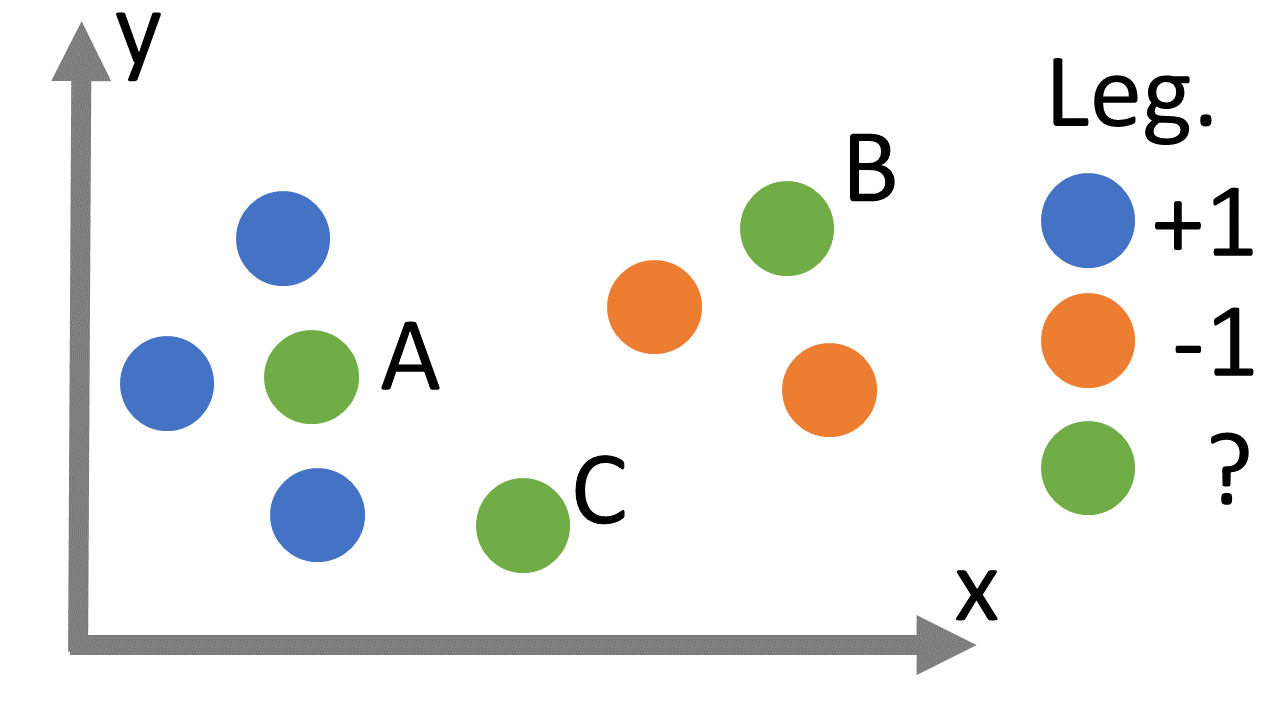
\includegraphics[width=0.5\linewidth]{PowerPoint/Folie1.png}
            % \caption{Beispiel eines Training-Sets mit zu klassifizierenden Punkten}
            \label{motivation:fig_1}
        }
    \end{figure}

    \vspace{3mm}

    \begin{itemize}
        \item Klassifizierung von Objekten
        \item Schnell und effizient
        \item Möglichst genau
    \end{itemize}
\end{frame}

%%%%%%%%%%%%%%%%%%%%%%%%%%%%%%%%%%%%%%%%%%%%%%%%%%%%%%%%%%%%%%%%%%%%%%%%%%%%%%%%
%Folie 2: Themenvorstellung
%%%%%%%%%%%%%%%%%%%%%%%%%%%%%%%%%%%%%%%%%%%%%%%%%%%%%%%%%%%%%%%%%%%%%%%%%%%%%%%%
\begin{frame}
    \frametitle{Themenvorstellung}

    \begin{figure}[h]
        \centering{
            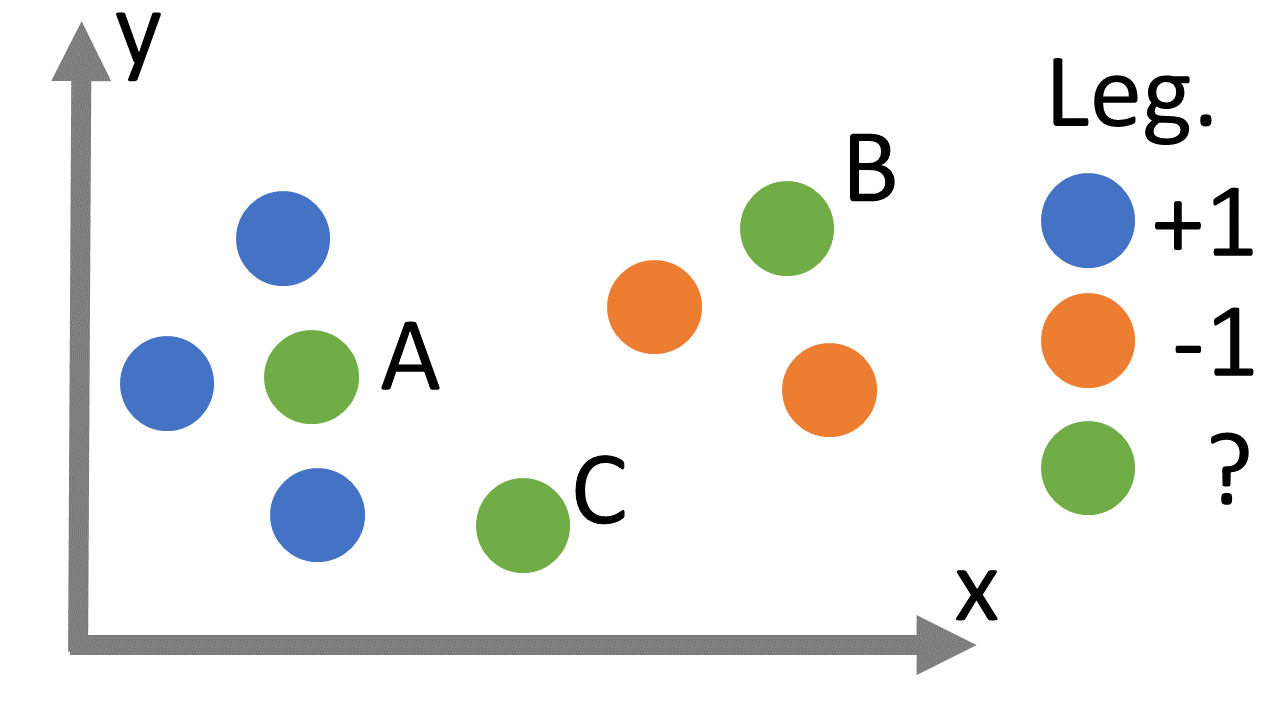
\includegraphics[width=0.5\linewidth]{PowerPoint/Folie1.png}
            % \caption{Beispiel eines Training-Sets mit zu klassifizierenden Punkten}
            \label{themenvorstellung:fig_1}
        }
    \end{figure}

    \vspace{3mm}

    \begin{itemize}
        \item Support Vector Machine
        \item Binärer Klassifizierer
    \end{itemize}
\end{frame}

%%%%%%%%%%%%%%%%%%%%%%%%%%%%%%%%%%%%%%%%%%%%%%%%%%%%%%%%%%%%%%%%%%%%%%%%%%%%%%%%
%Folie 3: Inhalt
%%%%%%%%%%%%%%%%%%%%%%%%%%%%%%%%%%%%%%%%%%%%%%%%%%%%%%%%%%%%%%%%%%%%%%%%%%%%%%%%
\begin{frame}
    \frametitle{Inhalt}

    \begin{itemize}
        \item Grundlagen von SVM
        \item Kernel-Trick
        \item Praxis mit Python
    \end{itemize}
\end{frame}

%%%%%%%%%%%%%%%%%%%%%%%%%%%%%%%%%%%%%%%%%%%%%%%%%%%%%%%%%%%%%%%%%%%%%%%%%%%%%%%%
%Folie 4: Problemstellung
%%%%%%%%%%%%%%%%%%%%%%%%%%%%%%%%%%%%%%%%%%%%%%%%%%%%%%%%%%%%%%%%%%%%%%%%%%%%%%%%
\begin{frame}
    \frametitle{Problemstellung}

    \only<1>{
        \begin{figure}[h]
            \centering{
                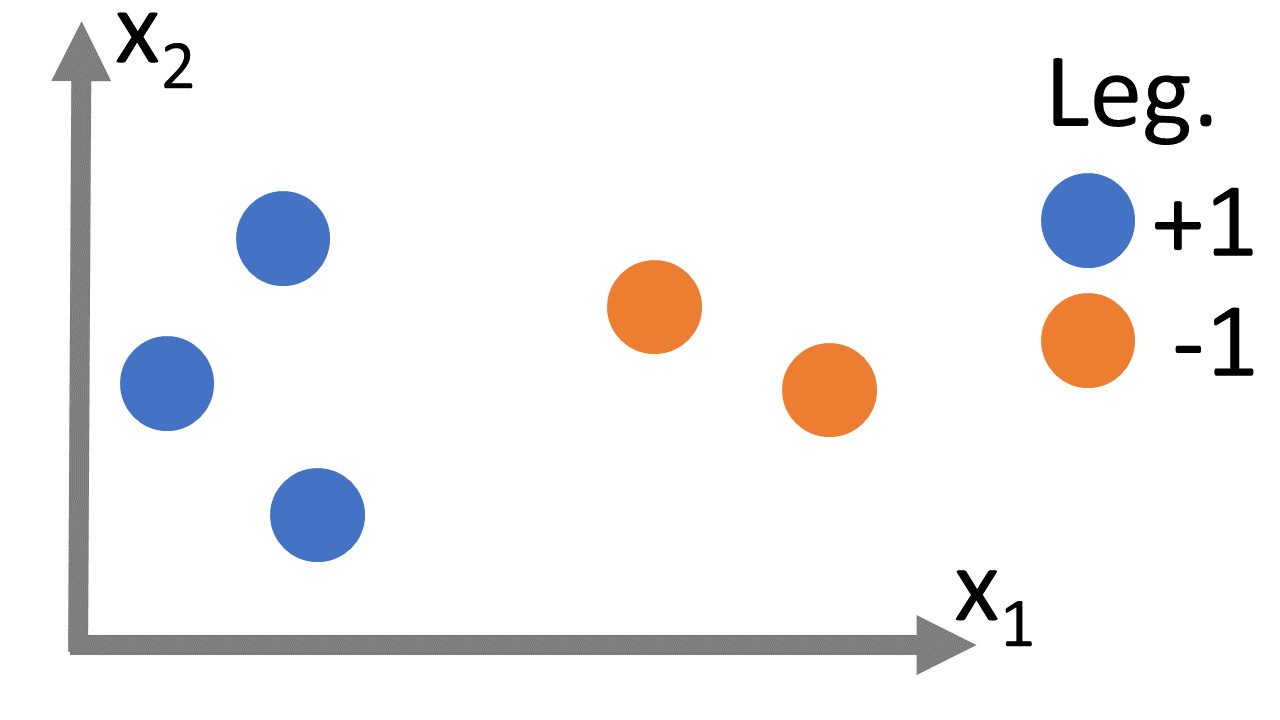
\includegraphics[width=0.5\textwidth]{PowerPoint/Folie2.png}
                % \caption{Beispiel eines Training-Sets}
                \label{lin_klassif:fig_1}
            }
        \end{figure}

        \vspace{3mm}

        \begin{itemize}
            \item Wie trenne ich die beiden Klassen voneinander?
        \end{itemize}
    }\only<2-3>{
        \begin{figure}[h]
            \begin{minipage}{0.4\textwidth} 
                \begin{figure}[h]
                    \centering{
                        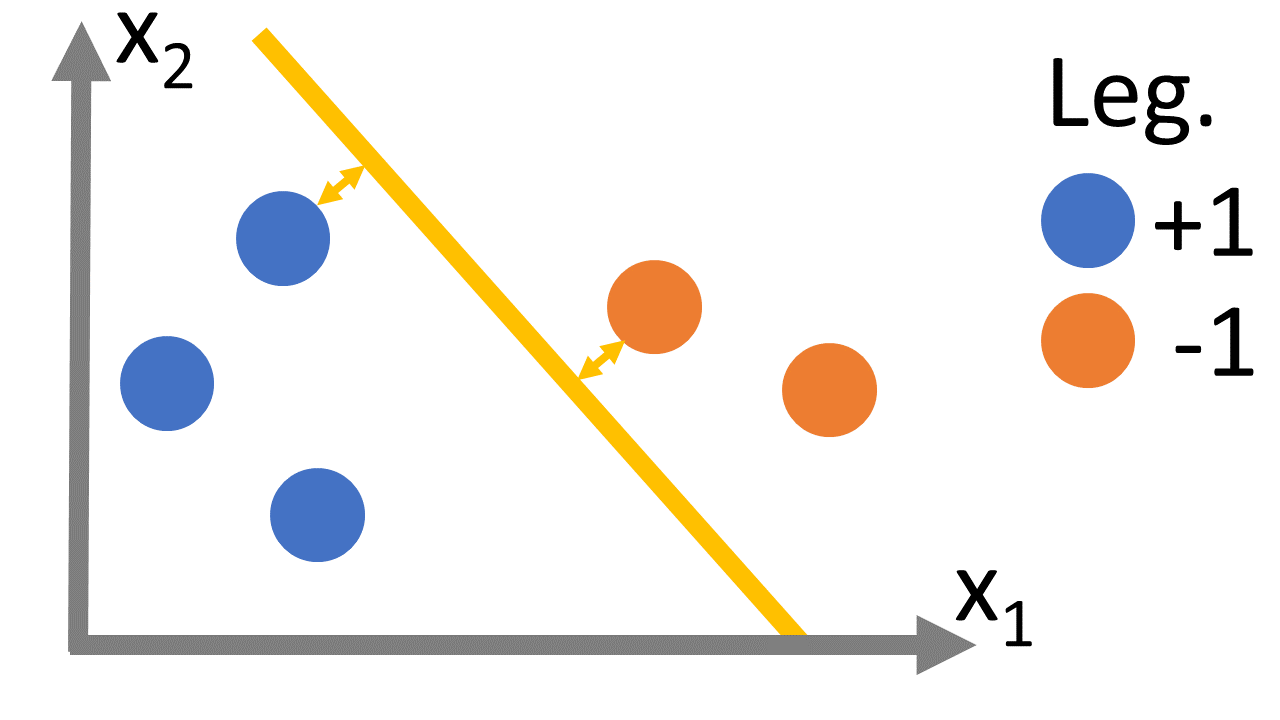
\includegraphics[width=\textwidth]{PowerPoint/Folie3.png}
                        % \caption{Beispiel eines Training-Sets}
                        \label{definitionen:fig_2}
                    }
                \end{figure}
            \end{minipage}
            \hfill
            \begin{minipage}{0.4\textwidth}
                \begin{figure}[h]
                    \centering{
                        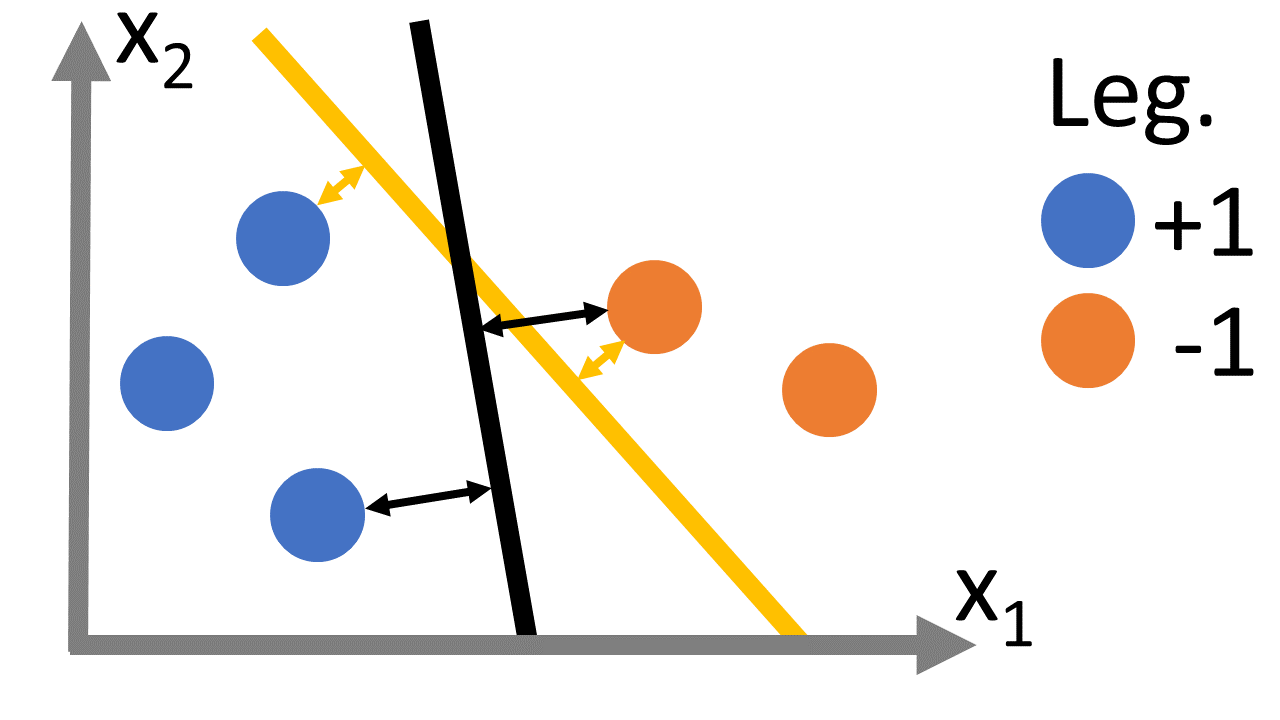
\includegraphics[width=\textwidth]{PowerPoint/Folie4.png}
                        % \caption{Beispiel eines Training-Sets}
                        \label{definitionen:fig_3}
                    }
                \end{figure}
            \end{minipage}
        \end{figure}

        \vspace{2mm}

        \begin{itemize}
            \item<2-> Wie lege ich die Hyperebene am besten?

            \item<3-> Anderer Name von Support Vector Machines: Large Margin Classifier
        \end{itemize}
    }
\end{frame}

%%%%%%%%%%%%%%%%%%%%%%%%%%%%%%%%%%%%%%%%%%%%%%%%%%%%%%%%%%%%%%%%%%%%%%%%%%%%%%%%
%Folie 5: Support vectors
%%%%%%%%%%%%%%%%%%%%%%%%%%%%%%%%%%%%%%%%%%%%%%%%%%%%%%%%%%%%%%%%%%%%%%%%%%%%%%%%
\begin{frame}
    \frametitle{Support vectors (s.v.)}

    \begin{figure}[h]
        \begin{minipage}{0.4\textwidth} 
            \begin{figure}[h]
                \centering{
                    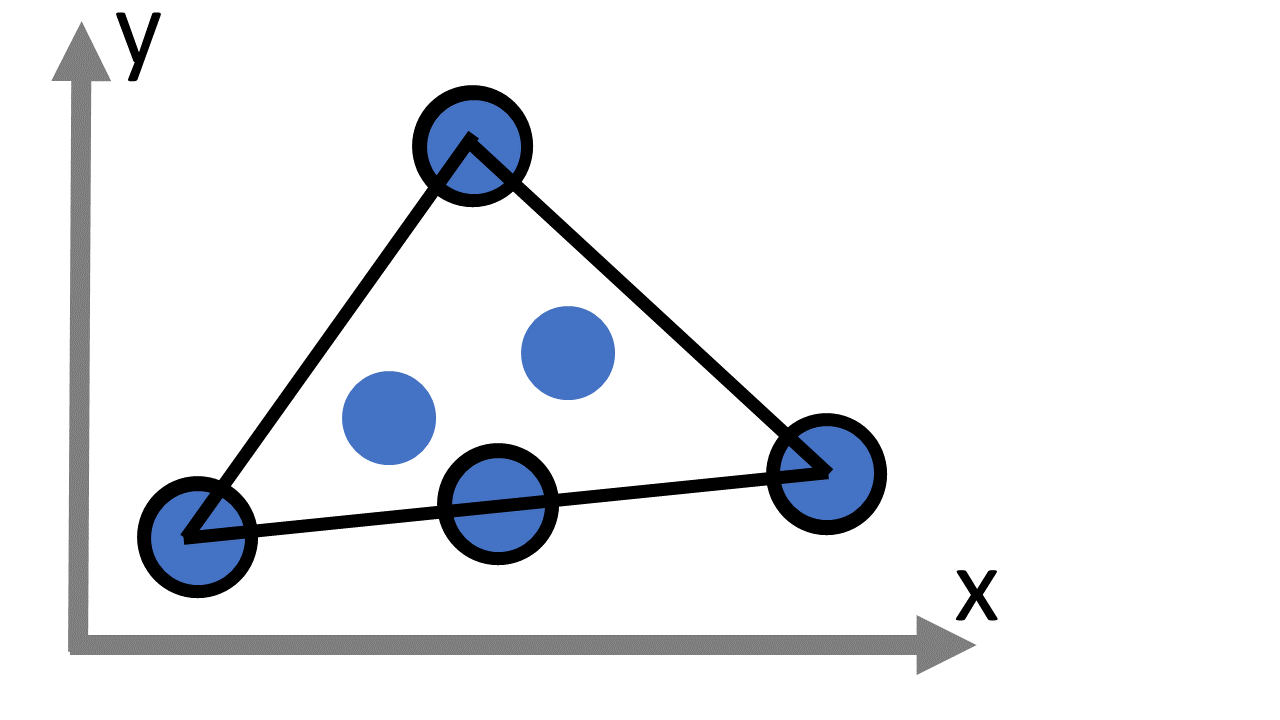
\includegraphics[width=\textwidth]{PowerPoint/Folie14.png}
                    % \caption{Beispiel eines Training-Sets}
                    \label{sv:fig_1}
                }
            \end{figure}
        \end{minipage}
        \hfill
        \begin{minipage}{0.4\textwidth}
            \begin{figure}[h]
                \centering{
                    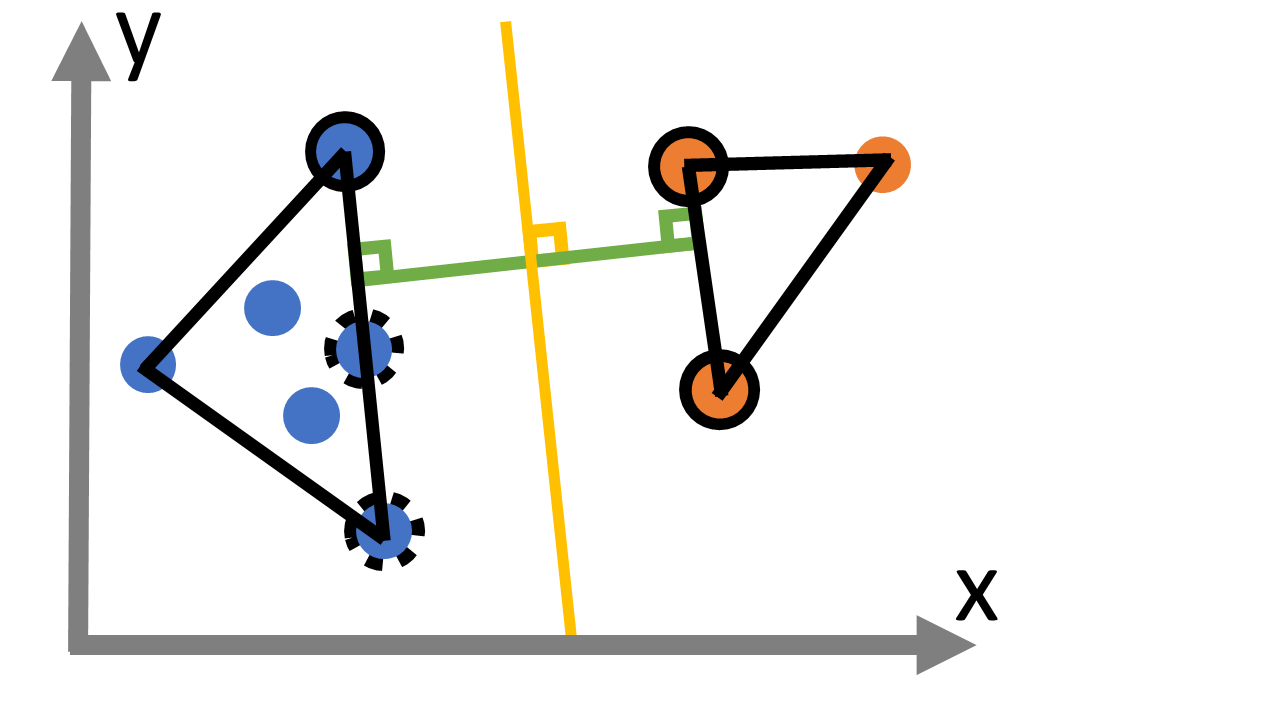
\includegraphics[width=\textwidth]{PowerPoint/Folie16.png}
                    % \caption{Beispiel eines Training-Sets}
                    \label{sv:fig_3}
                }
            \end{figure}
        \end{minipage}
    \end{figure}
    \begin{figure}[h]
        \begin{minipage}{0.4\textwidth} 
            \begin{figure}[h]
                \centering{
                    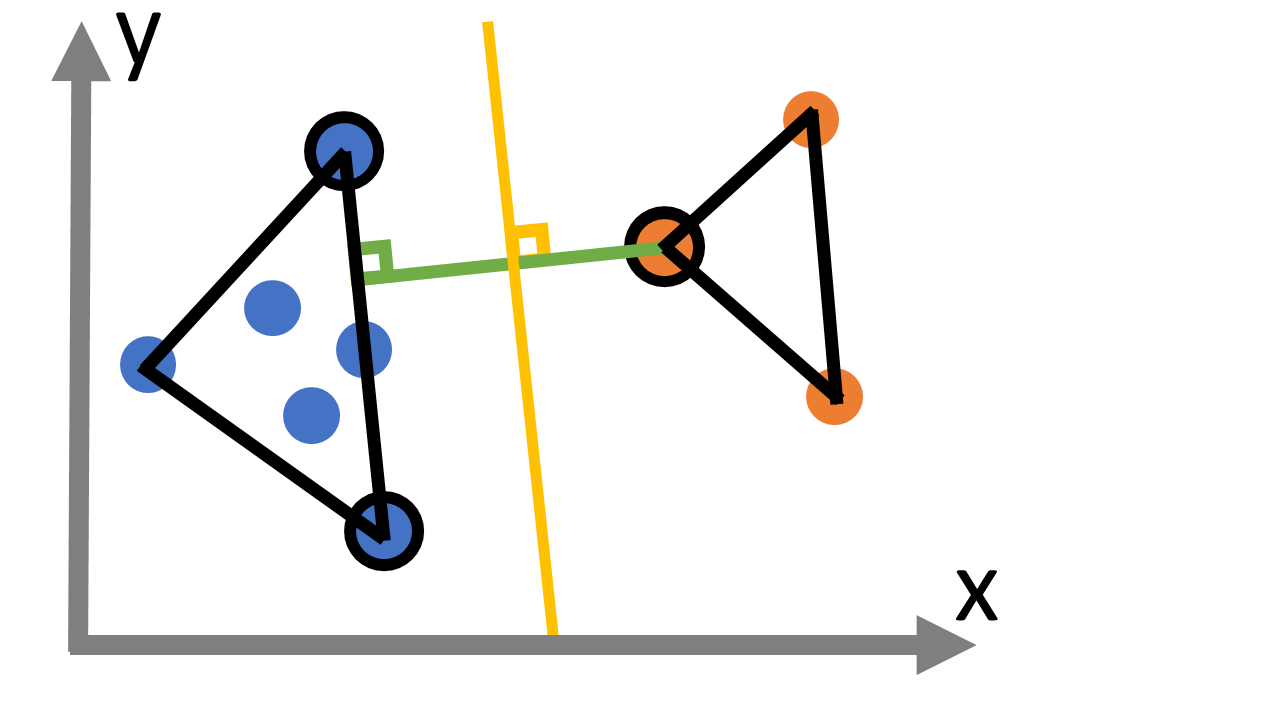
\includegraphics[width=\textwidth]{PowerPoint/Folie15.png}
                    % \caption{Beispiel eines Training-Sets}
                    \label{sv:fig_2}
                }
            \end{figure}
        \end{minipage}
        \hfill
        \begin{minipage}{0.4\textwidth}
            \begin{figure}[h]
                \centering{
                    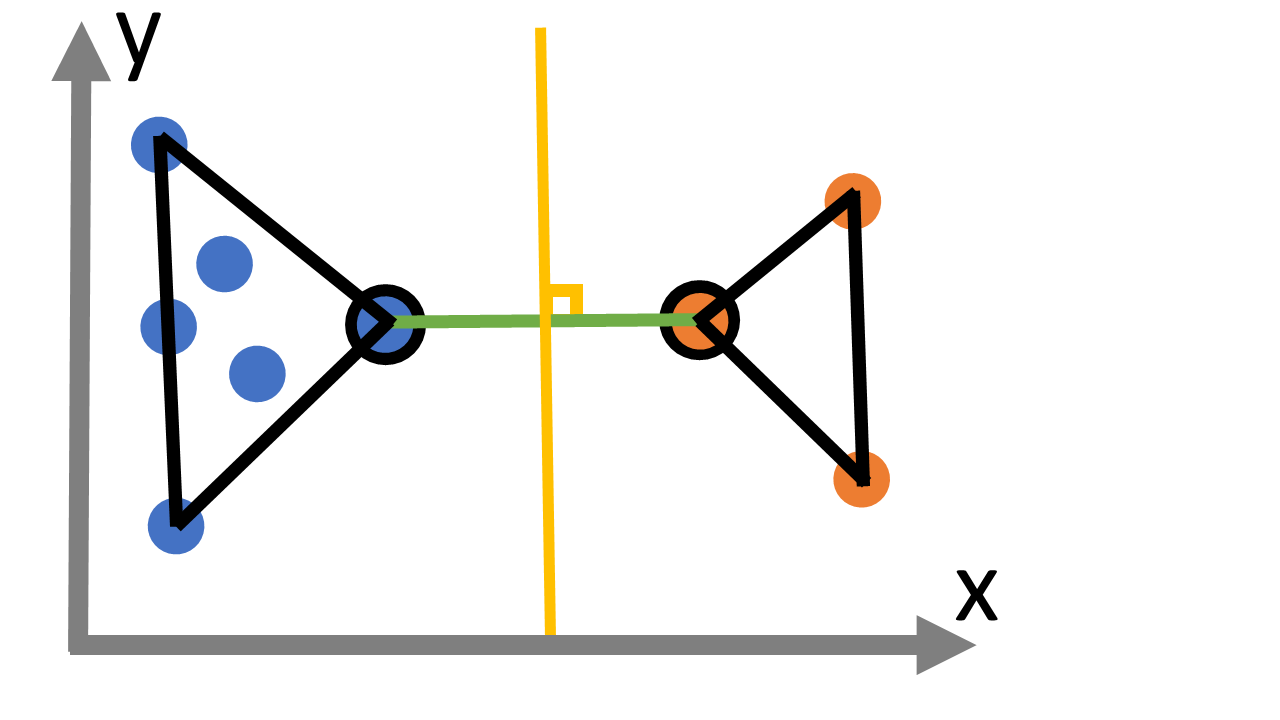
\includegraphics[width=\textwidth]{PowerPoint/Folie17.png}
                    % \caption{Beispiel eines Training-Sets}
                    \label{sv:fig_4}
                }
            \end{figure}
        \end{minipage}
    \end{figure}

\end{frame}

%%%%%%%%%%%%%%%%%%%%%%%%%%%%%%%%%%%%%%%%%%%%%%%%%%%%%%%%%%%%%%%%%%%%%%%%%%%%%%%%
%Folie 6: Definitionen
%%%%%%%%%%%%%%%%%%%%%%%%%%%%%%%%%%%%%%%%%%%%%%%%%%%%%%%%%%%%%%%%%%%%%%%%%%%%%%%%
\begin{frame}
    \frametitle{Definitionen}

    \begin{itemize}
        \item $ m \in \mathbb{R} $ Datenpunkte
        \item Input $ \boldsymbol{x} \in \mathbb{R}^N $
        % \item Input $ \boldsymbol{x} := \{ \boldsymbol{x}_1, \dots, \boldsymbol{x}_m \} \text{, } \boldsymbol{x} \in \mathbb{R}^N $
        \item Output $ y \in \{ -1, +1 \} $
        \item Trainingsset $S \in (\mathbb{R}^N \times \{ -1, +1 \})^m $
    \end{itemize}

    \vspace{2mm}

    \begin{itemize}
        \item Hypothese
            \begin{align*}
                h: \mathbb{R}^N &\to \{ +1, -1 \} \\
                \boldsymbol{x} &\mapsto y \\
            \end{align*}
    \end{itemize}

    \vspace{3mm}

    \begin{figure}[h]
        \begin{minipage}{0.4\textwidth} 
            \begin{figure}[h]
                \centering{
                    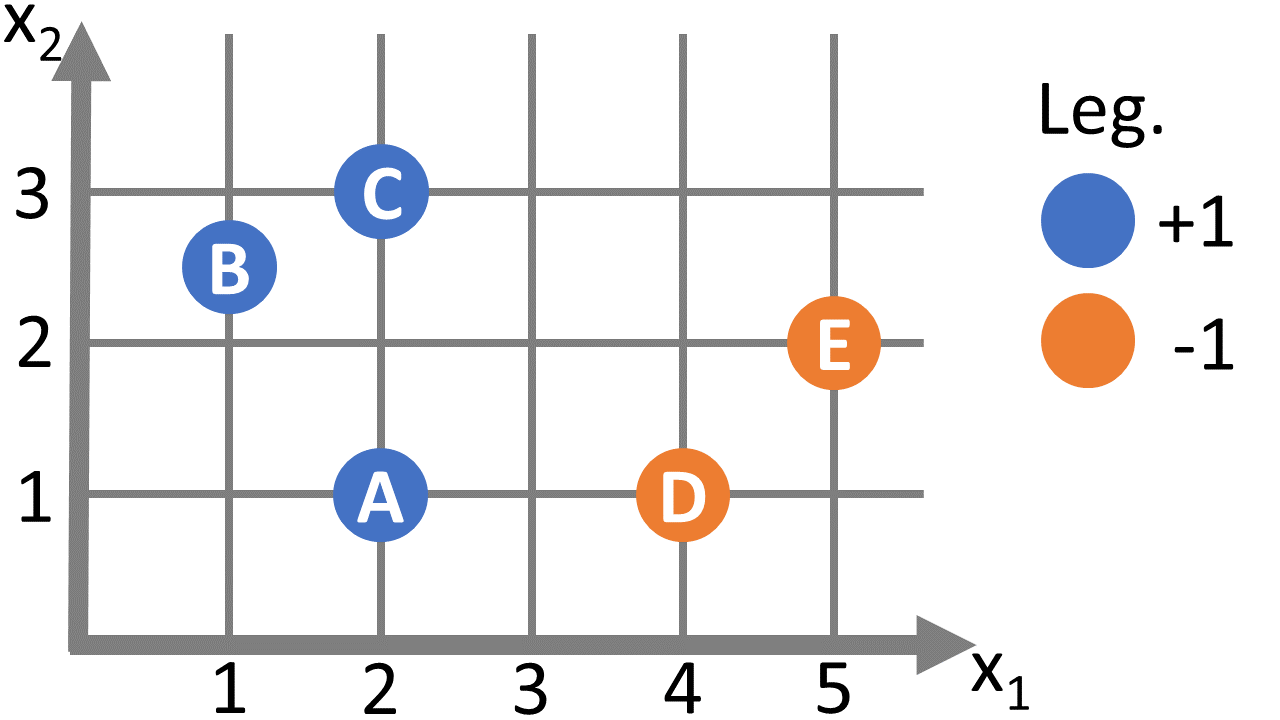
\includegraphics[width=\textwidth]{PowerPoint/Folie9.png}
                    % \caption{Beispiel eines Training-Sets}
                    \label{definitionen:fig_1}
                }
            \end{figure}
        \end{minipage}
        \hfill
        \begin{minipage}{0.4\textwidth}
            \begin{itemize}
                \item<2-> $m = 5$
                \item<2-> Trainingsset $S$:
                    \begin{align*}
                        S = \left( \begin{matrix}
                            1 & 2.5 & +1 \\
                            5 & 2 & -1 \\
                            & \vdots & \\
                        \end{matrix} \right) \\
                    \end{align*}
            \end{itemize} 
        \end{minipage}
    \end{figure}
\end{frame}

%%%%%%%%%%%%%%%%%%%%%%%%%%%%%%%%%%%%%%%%%%%%%%%%%%%%%%%%%%%%%%%%%%%%%%%%%%%%%%%%
%Folie 7: Verlauf der Hyperbene
%%%%%%%%%%%%%%%%%%%%%%%%%%%%%%%%%%%%%%%%%%%%%%%%%%%%%%%%%%%%%%%%%%%%%%%%%%%%%%%%
\begin{frame}
    \frametitle{Verlauf der Hyperbene}

    \begin{figure}[h]
        \centering{
            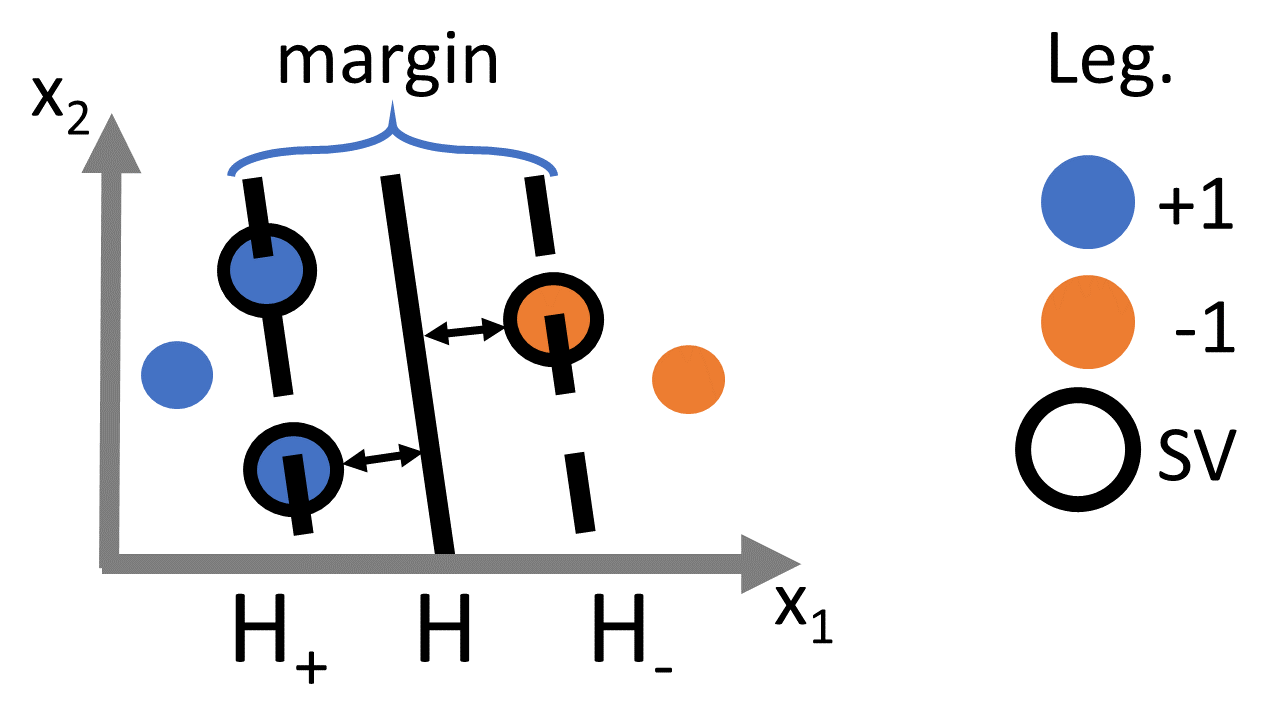
\includegraphics[width=0.5\textwidth]{PowerPoint/Folie7.png}
            % \caption{Beispiel eines Training-Sets}
            \label{large_marg_class:fig_1}
        }
    \end{figure}

    \vspace{3mm}

    \only<1> {
        \begin{itemize}
            \item Hyperebene: $ H' = \boldsymbol{w}'^T \boldsymbol{x} + b' = 0 $
            \item Gutter: $H_+$ und $H_-$
            \item Hyperbene frei skalierbar
        \end{itemize}
    }\only<2> {
        \begin{itemize}
            \item Hyperebene: $ H' = \boldsymbol{w}'^T \boldsymbol{x} + b' = 0 $
            \item Gutter constraint (GC):
                \begin{align*}
                    H_+ := & \boldsymbol{w}^T \boldsymbol{x}_p + b = +1, \quad \forall \text{ s.v., die auf } H_+ \text{ liegen} \\
                    H_- := & \boldsymbol{w}^T \boldsymbol{x}_n + b = -1, \quad \forall \text{ s.v., die auf } H_- \text{ liegen} \\
                    & y_i ( \boldsymbol{w}^T \boldsymbol{x}_i + b ) = 1 \quad \forall \text{ s.v. } \\
                \end{align*}
            \item Um GC zu erfüllen: $ \boldsymbol{w} $ und $b$ werden um $ v \in \mathbb{R} $ skaliert:
                \begin{align*}
                    & \boldsymbol{w} = v^T \boldsymbol{w}' & b = v^T b' \\
                    & H = v ( \boldsymbol{w}^T \boldsymbol{x} + b ) = 0
                \end{align*} \\
            \item $H$ heißt auch kanonische Hyperebene
        \end{itemize}
    }\only<3> {
        \begin{itemize}
            \item Kanonische Hyperebene: $ H = \boldsymbol{w}^T \boldsymbol{x} + b = 0 $
            \item Kanonische Hyperebene ermöglicht Klassifizierung:
                \begin{equation*}
                    h(x_i) = \begin{cases}
                        +1 & \text{ wenn } \boldsymbol{w}^T \boldsymbol{x}_i + b \geq 0 \\
                        -1 & \text{ wenn } \boldsymbol{w}^T \boldsymbol{x}_i + b \leq 0 \\
                    \end{cases}
                \end{equation*}
        \end{itemize}
    }
\end{frame}

%%%%%%%%%%%%%%%%%%%%%%%%%%%%%%%%%%%%%%%%%%%%%%%%%%%%%%%%%%%%%%%%%%%%%%%%%%%%%%%%
% Folie 8: Beispiel I
%%%%%%%%%%%%%%%%%%%%%%%%%%%%%%%%%%%%%%%%%%%%%%%%%%%%%%%%%%%%%%%%%%%%%%%%%%%%%%%%
\begin{frame}
    \frametitle{Beispiel I}

    \begin{figure}[h]
        \begin{minipage}{0.4\textwidth} 
            \only<1>{
                \begin{figure}[h]
                    \centering{
                        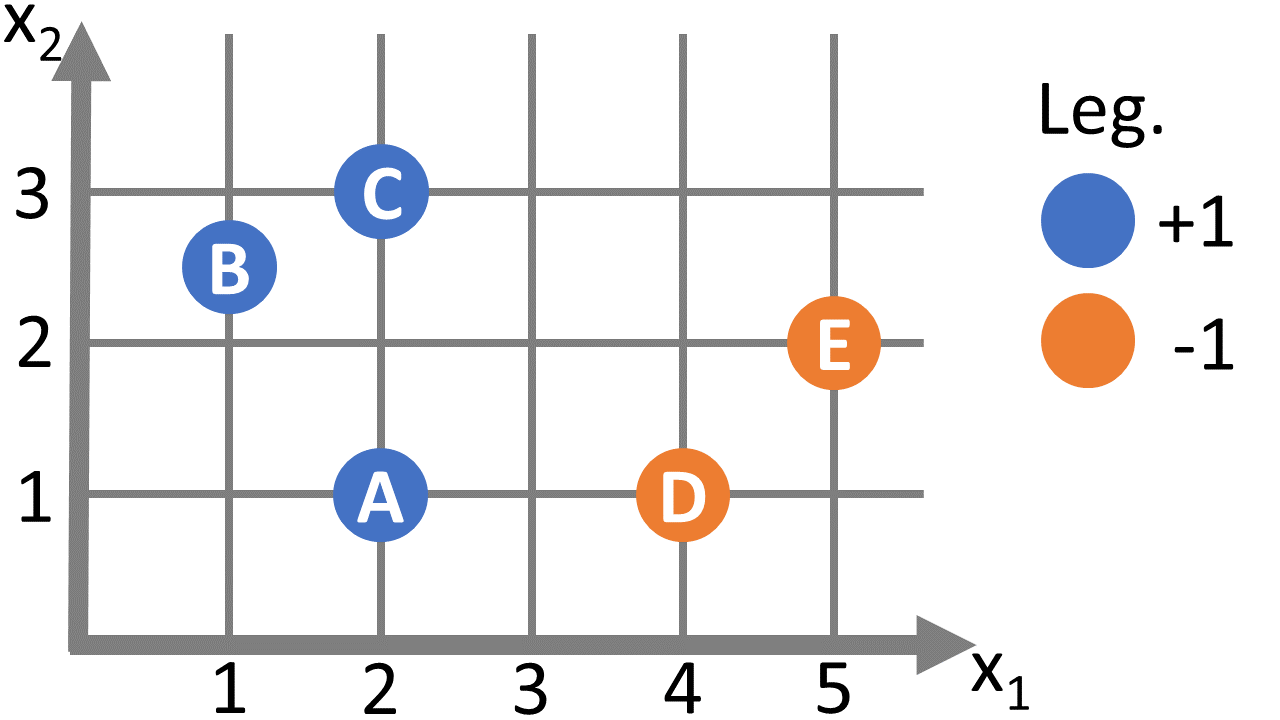
\includegraphics[width=\textwidth]{PowerPoint/Folie9.png}
                        % \caption{Beispiel eines Training-Sets}
                        \label{Bsp_1:fig_1}
                    }
                \end{figure}
            }\only<2->{
                \begin{figure}[h]
                    \centering{
                        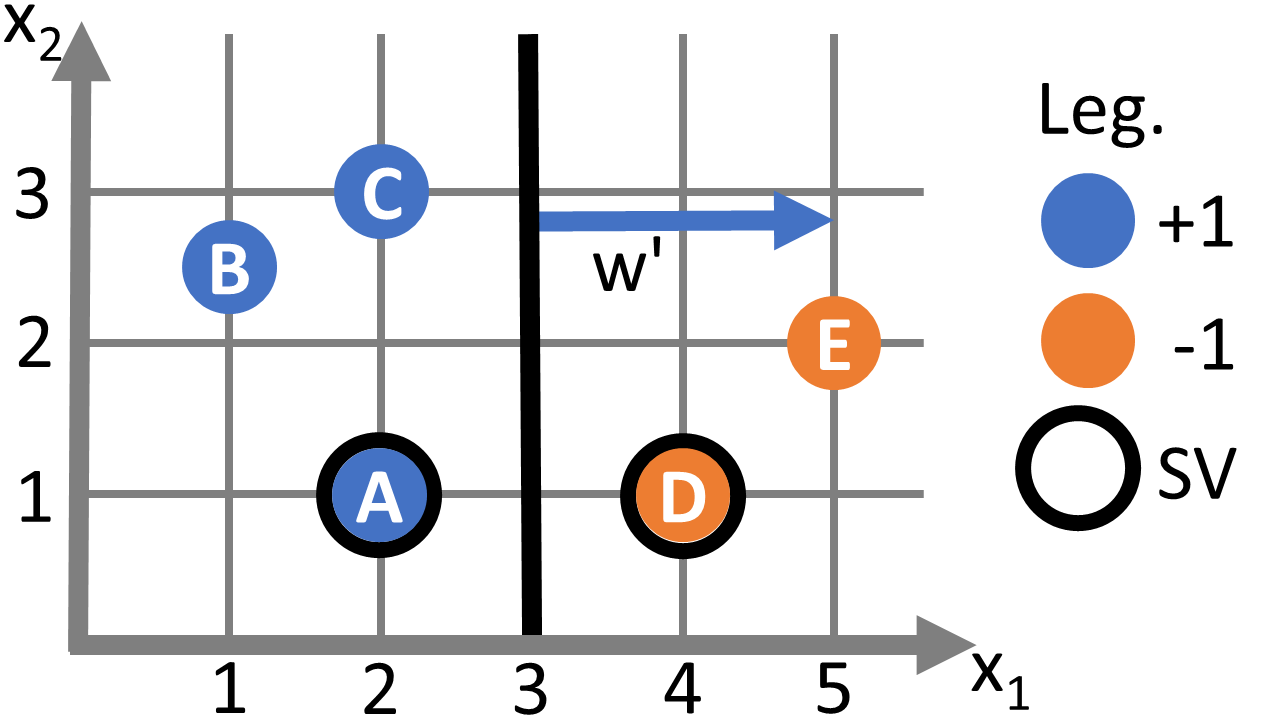
\includegraphics[width=\textwidth]{PowerPoint/Folie10.png}
                        % \caption{Beispiel eines Training-Sets}
                        \label{Bsp_1:fig_2}
                    }
                \end{figure}
            }
        \end{minipage}
        \hfill
        \begin{minipage}{0.4\textwidth}
            \begin{itemize}
                \item<1-> Hyperebene: $ H = \boldsymbol{w}^T \boldsymbol{x} + b = 0 $
                \item<1-> Gutter constraint: $ \boldsymbol{w}^T \boldsymbol{x}_i + b = y_i, \quad \forall \text{ s. v. } \in \boldsymbol{x} $
            \end{itemize} 
        \end{minipage}
    \end{figure}

    \begin{itemize}
        \item <2-> Graphische Bestimmung der Hyperebenenparameter:
            \begin{align*}
                x &= 3 \\
                \boldsymbol{w} &= \left( \begin{matrix}
                    2 \\
                    0 \\
                \end{matrix} \right) \\
                \left( \begin{matrix}
                    2 & 0 \\
                \end{matrix} \right)^T \left( \begin{matrix}
                    3 \\
                    0 \\
                \end{matrix} \right) + b = 0 &\Rightarrow b = -6 \\
            \end{align*}
    \end{itemize}
\end{frame}

%%%%%%%%%%%%%%%%%%%%%%%%%%%%%%%%%%%%%%%%%%%%%%%%%%%%%%%%%%%%%%%%%%%%%%%%%%%%%%%%
% Folie 9: Beispiel II
%%%%%%%%%%%%%%%%%%%%%%%%%%%%%%%%%%%%%%%%%%%%%%%%%%%%%%%%%%%%%%%%%%%%%%%%%%%%%%%%
\begin{frame}
    \frametitle{Beispiel II}

    \begin{figure}[h]
        \begin{minipage}{0.4\textwidth} 
            \only<1>{
                \begin{figure}[h]
                    \centering{
                        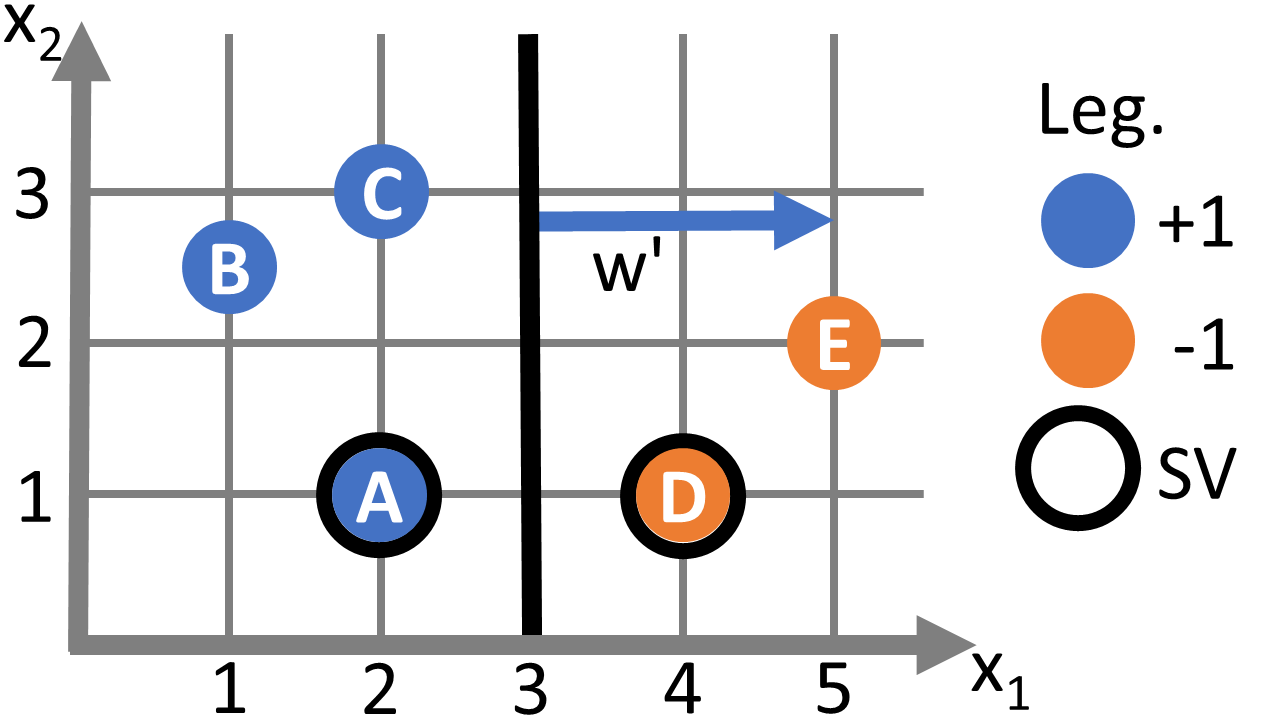
\includegraphics[width=\textwidth]{PowerPoint/Folie10.png}
                        % \caption{Beispiel eines Training-Sets}
                        \label{Bsp_1:fig_2}
                    }
                \end{figure}
            }\only<2->{
                \begin{figure}[h]
                    \centering{
                        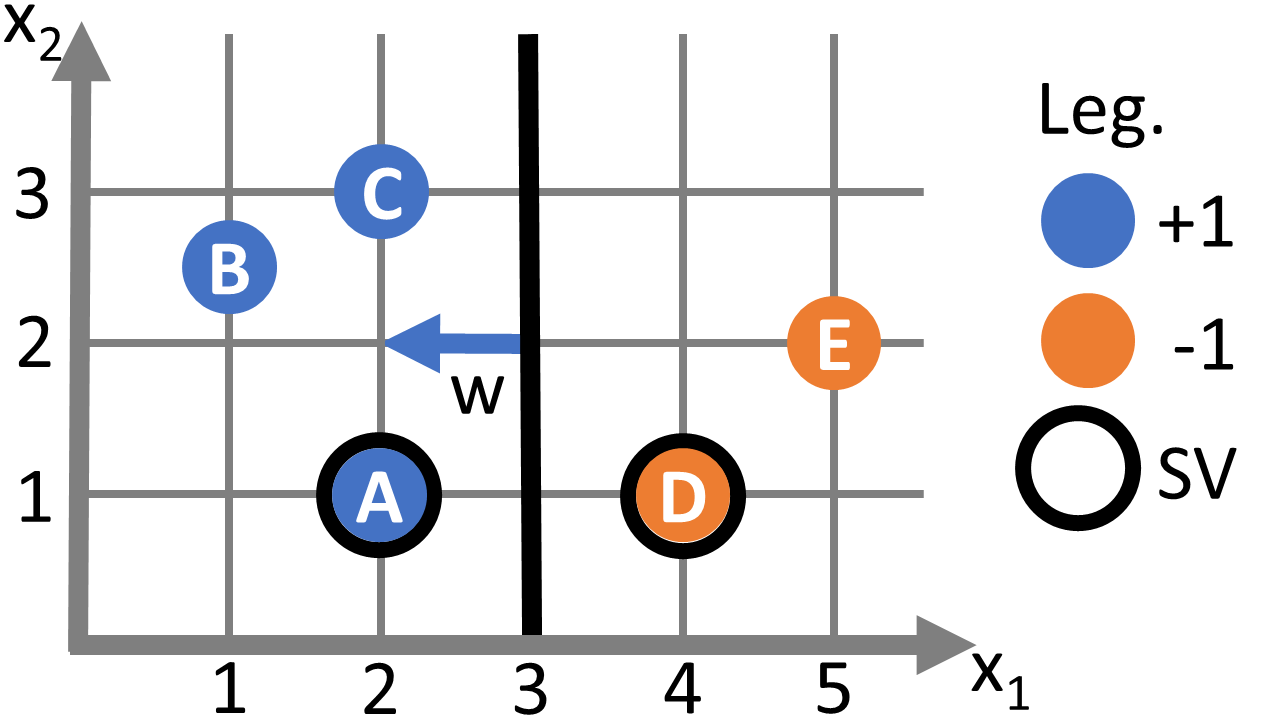
\includegraphics[width=\textwidth]{PowerPoint/Folie11.png}
                        % \caption{Beispiel eines Training-Sets}
                        \label{Bsp_1:fig_2}
                    }
                \end{figure}
            }
        \end{minipage}
        \hfill
        \begin{minipage}{0.4\textwidth}
            \begin{itemize}
                \item<1-> Hyperebene: $ H = \boldsymbol{w}^T \boldsymbol{x} + b = 0 $
                \item<1-> Gutter constraint: $ \boldsymbol{w}^T \boldsymbol{x}_i + b = y_i, \quad \forall \text{ s. v. } \in \boldsymbol{x} $
            \end{itemize} 
        \end{minipage}
    \end{figure}

    \begin{itemize}
        \item<1-> Berücksichtigen der Gutter constraint am Bsp. von Punkt $A$:
            \begin{align*}
                c \left( \left( \begin{matrix}
                    2 & 0 \\
                \end{matrix} \right)^T \left( \begin{matrix}
                    2 \\
                    1 \\
                \end{matrix} \right) - 6 \right) \overset{!}{=} +1 &\Rightarrow c = -0.5 \\
            \end{align*}
        \item<2-> Somit gilt für die kanonische Hyperebene:
            \begin{align*}
                \boldsymbol{w} &= \left( \begin{matrix}
                    -1 \\
                    0 \\
                \end{matrix} \right) \\
                b &= 3 \\ 
            \end{align*}
        \item<3-> Kontrolle mit Punkt $D$:
            \begin{align*}
                \left( \begin{matrix}
                    -1 & 0 \\
                \end{matrix} \right)^T \left( \begin{matrix}
                    4 \\
                    1 \\
                \end{matrix} \right) + 3 = -1
            \end{align*}
    \end{itemize}
\end{frame}

%%%%%%%%%%%%%%%%%%%%%%%%%%%%%%%%%%%%%%%%%%%%%%%%%%%%%%%%%%%%%%%%%%%%%%%%%%%%%%%%
% Folie 10: Beispiel III
%%%%%%%%%%%%%%%%%%%%%%%%%%%%%%%%%%%%%%%%%%%%%%%%%%%%%%%%%%%%%%%%%%%%%%%%%%%%%%%%
\begin{frame}
    \frametitle{Beispiel III}

    \begin{figure}[h]
        \begin{minipage}{0.4\textwidth} 
            \only<1->{
                \begin{figure}[h]
                    \centering{
                        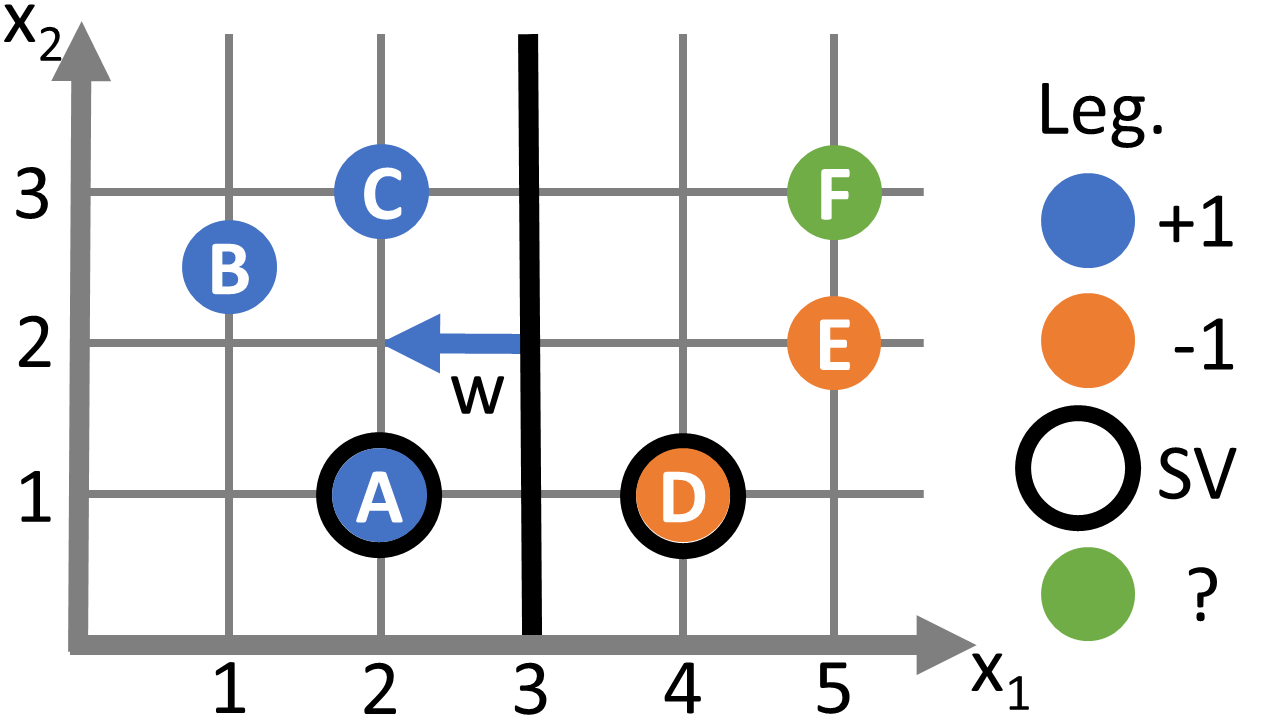
\includegraphics[width=\textwidth]{PowerPoint/Folie12.png}
                        % \caption{Beispiel eines Training-Sets}
                        \label{Bsp_1:fig_2}
                    }
                \end{figure}
            }
        \end{minipage}
        \hfill
        \begin{minipage}{0.4\textwidth}
            \begin{itemize}
                \item<1-> Klassifizierung:
                    \begin{equation*}
                        h(x_i) = \begin{cases}
                            +1 & \text{if } \boldsymbol{w}^T \boldsymbol{x}_i + b \geq 0 \\
                            -1 & \text{if } \boldsymbol{w}^T \boldsymbol{x}_i + b \leq 0 \\
                        \end{cases}
                    \end{equation*}
                \item<1-> Parameter der kanonischen Hyperebene
                    \begin{align*}
                        \boldsymbol{w} &= \left( \begin{matrix}
                            -1 \\
                            0 \\
                        \end{matrix} \right) \\
                        b &= 3 \\ 
                    \end{align*}
            \end{itemize} 
        \end{minipage}
    \end{figure}

    \begin{itemize}
        \item<1-> Klassifizierung von Punkt $F$:
            \begin{align*}
                \left( \begin{matrix}
                    -1 & 0 \\
                \end{matrix} \right)^T \left( \begin{matrix}
                    5 \\
                    3 \\
                \end{matrix} \right) + 3 = -2
            \end{align*}
        \item<1-> Punkt F gehört also zur Klasse $-1$.
    \end{itemize}
\end{frame}

%%%%%%%%%%%%%%%%%%%%%%%%%%%%%%%%%%%%%%%%%%%%%%%%%%%%%%%%%%%%%%%%%%%%%%%%%%%%%%%%
% Folie 11: Minimierungsproblem
%%%%%%%%%%%%%%%%%%%%%%%%%%%%%%%%%%%%%%%%%%%%%%%%%%%%%%%%%%%%%%%%%%%%%%%%%%%%%%%%
\begin{frame}
    \frametitle{Minimierungsproblem}

    \begin{figure}[h]
        \centering{
            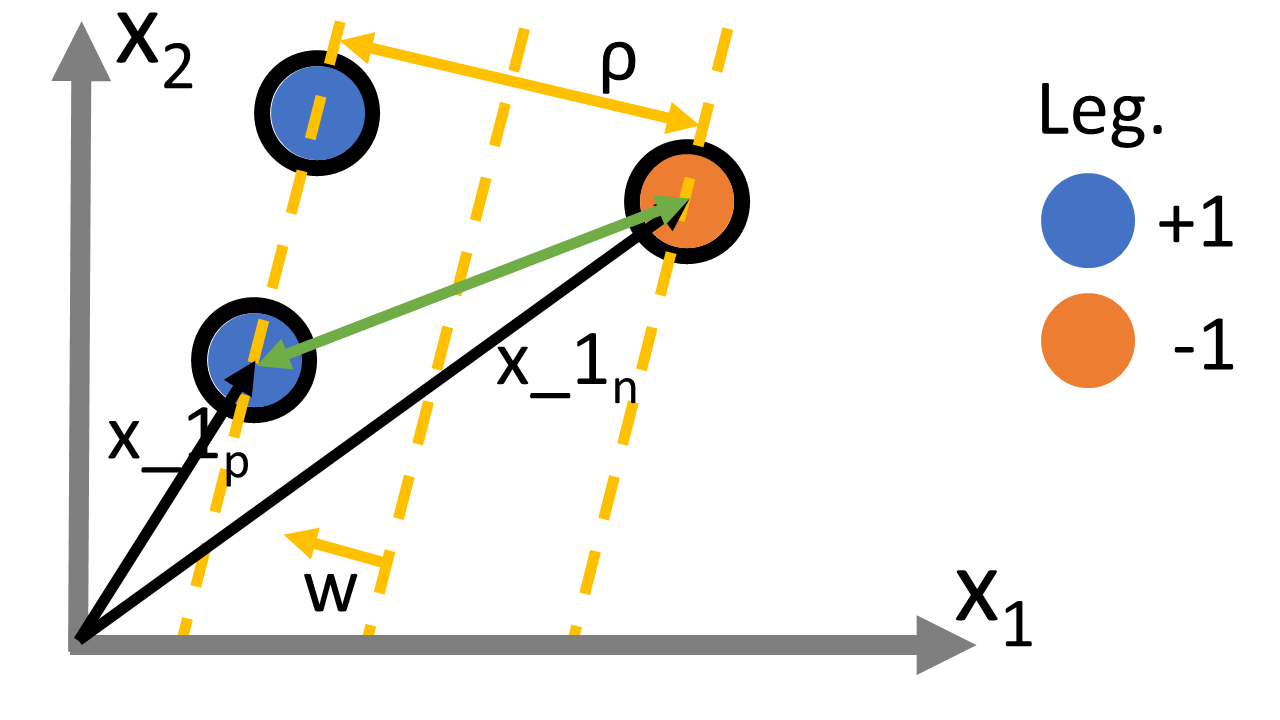
\includegraphics[width=0.5\textwidth]{PowerPoint/Folie8.png}
            % \caption{Beispiel eines Training-Sets}
            \label{Min_Prob:fig_1}
        }
    \end{figure}

    \only<1>{
        \begin{itemize}
            \item Projektionseigenschaft des Skalarprodukts
            \item Breite des margin $\rho$:
                \begin{equation*}
                    \rho = (\boldsymbol{x}_p - \boldsymbol{x}_n)^T \frac{\boldsymbol{w}}{\Vert \boldsymbol{w} \Vert} \Leftrightarrow \rho = (\boldsymbol{x}_p^T \boldsymbol{w} - \boldsymbol{x}_n^T \boldsymbol{w}) \frac{1}{\Vert \boldsymbol{w} \Vert}
                \end{equation*}
            \item Gutter constraint: 
                \begin{align*}
                    y_i ( \boldsymbol{w}^T \boldsymbol{x}_i + b ) = 1 \quad \forall \text{ s.v. } \in \boldsymbol{x}
                \end{align*}
            \item $ \rho = \frac{2}{\Vert \boldsymbol{w} \Vert} $
            \item Ziel einer SVM: Maximiere den margin
                \begin{align*}
                    & \max_{\boldsymbol{w}, b} \frac{2}{\Vert \boldsymbol{w} \Vert} \Leftrightarrow \min_{\boldsymbol{w}, b} \Vert \boldsymbol{w} \Vert \Leftrightarrow \min_{\boldsymbol{w}, b} \frac{1}{2} \Vert \boldsymbol{w} \Vert^2 \\
                    & \text{u.d.N. } y_i ( \boldsymbol{w}^T \boldsymbol{x}_i + b ) - 1 \geq 0 \\
                \end{align*}
        \end{itemize} 
    }
\end{frame}

%%%%%%%%%%%%%%%%%%%%%%%%%%%%%%%%%%%%%%%%%%%%%%%%%%%%%%%%%%%%%%%%%%%%%%%%%%%%%%%%
% Folie 12: Lagrange Multiplikatoren
%%%%%%%%%%%%%%%%%%%%%%%%%%%%%%%%%%%%%%%%%%%%%%%%%%%%%%%%%%%%%%%%%%%%%%%%%%%%%%%%
\begin{frame}
    \frametitle{Lagrange Multiplikatoren}

    \begin{itemize}
        \item Langrange Multiplikatoren:
            \begin{align*}
                L = \frac{1}{2} \Vert \boldsymbol{w} \Vert^2 - \sum \alpha_i \left[ y_i ( \boldsymbol{w}^T \boldsymbol{x}_i + b) - 1 \right] \\
            \end{align*}
        \item Suche nach den Extremum
            \begin{align*}
                \frac{\partial L}{\partial \boldsymbol{w}} = \boldsymbol{w} - \sum \alpha_i y_i \boldsymbol{x}_i = 0 &\Rightarrow \boldsymbol{w} = \sum_i \alpha_i y_i \boldsymbol{x}_i \\
                \frac{\partial L}{\partial b} = -\sum \alpha_i y_i = 0 &\Rightarrow \sum_i \alpha_i y_i = 0 \\
            \end{align*}
        \item $\boldsymbol{w}$ in $L$ eingesetzt:
            \begin{align*}
                L &= \frac{1}{2} (\sum_i \alpha_i y_i \boldsymbol{x}_i)^T (\sum_j \alpha_j y_j \boldsymbol{x}_j) - (\sum_i \alpha_i y_i \boldsymbol{x}_i)^T (\sum_j \alpha_j y_j \boldsymbol{x}_j) - \sum_i \alpha_i y_i b + \sum_i \alpha_i \\
                L &= \sum_i \alpha_i - \frac{1}{2} \sum_i \sum_j \alpha_i \alpha_j y_i y_j \boldsymbol{x}_i^T \boldsymbol{x}_j
            \end{align*}
        \item Ziel: $ \max_{\boldsymbol{w}, b, \boldsymbol{\alpha}} L$
        \item Entscheidungsfunktion:
            \begin{align*}
                h(\boldsymbol{x}) = \begin{cases}
                    +1 & \sum_i \alpha_i y_i \boldsymbol{x}_i^T \boldsymbol{x} + b \geq 0 \\
                    -1 & \sum_i \alpha_i y_i \boldsymbol{x}_i^T \boldsymbol{x} + b \leq 0 \\
                \end{cases}
            \end{align*}
    \end{itemize}
\end{frame}

%%%%%%%%%%%%%%%%%%%%%%%%%%%%%%%%%%%%%%%%%%%%%%%%%%%%%%%%%%%%%%%%%%%%%%%%%%%%%%%%
% Folie 13: Unterstützungsvariablen
%%%%%%%%%%%%%%%%%%%%%%%%%%%%%%%%%%%%%%%%%%%%%%%%%%%%%%%%%%%%%%%%%%%%%%%%%%%%%%%%
\begin{frame}
    \frametitle{Unterstützungsvariablen $\alpha$}

    \begin{itemize}
        \item Eigenschaften:
            \begin{align*}
                & \boldsymbol{\alpha} \geq 0 & \alpha_i \begin{cases}
                    > 0 & \text{ wenn } x_i \text{ ein support vector ist} \\
                    = 0 & \text{ sonst} \\
                \end{cases} \\
                & \sum\limits_{\substack{ \text{pos. s.v.} \\ p}} \alpha_p  = \sum\limits_{\substack{ \text{neg. s.v.} \\ n}} \alpha_n \\
            \end{align*}
    \end{itemize}

    \vspace{3mm}

    \only<2>{
        \begin{figure}[h]
            \begin{minipage}{0.4\textwidth} 
                \begin{figure}[h]
                    \centering{
                        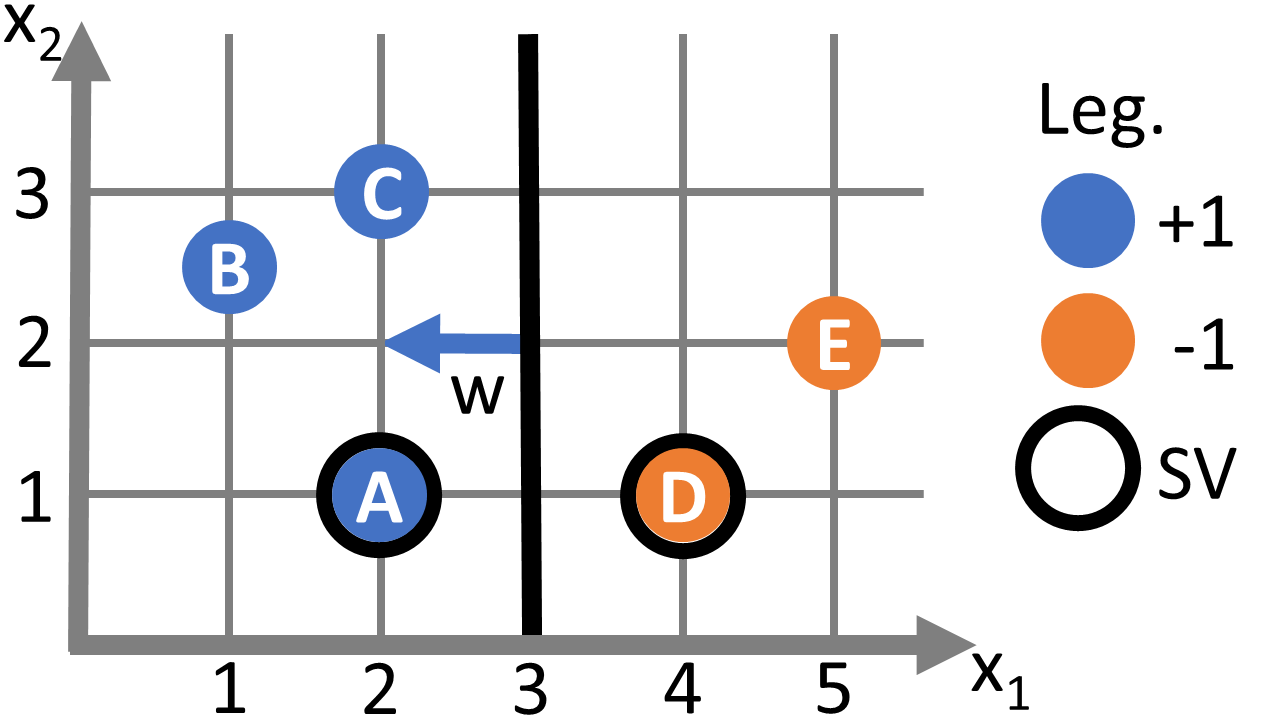
\includegraphics[width=\textwidth]{PowerPoint/Folie11.png}
                        % \caption{Beispiel eines Training-Sets}
                        \label{Bsp_1:fig_2}
                    }
                \end{figure}
            \end{minipage}
            \hfill
            \begin{minipage}{0.4\textwidth}
                \begin{itemize}
                    \item Berechnung von $\alpha_A$ und $\alpha_D$ ergibt:
                        \begin{align*}
                            \alpha_A &= 0.5 \\
                            \alpha_D &= 0.5
                        \end{align*}
                \end{itemize}

                \begin{itemize}
                    \item Berechnung von $\alpha_C$ ergibt:
                        \begin{align*}
                            \alpha_C = 0
                        \end{align*}
                \end{itemize}
            \end{minipage}
        \end{figure}
    }
\end{frame}

%%%%%%%%%%%%%%%%%%%%%%%%%%%%%%%%%%%%%%%%%%%%%%%%%%%%%%%%%%%%%%%%%%%%%%%%%%%%%%%%
% Folie 14: Ausgleich eines fehlerhaften Trainigssets
%%%%%%%%%%%%%%%%%%%%%%%%%%%%%%%%%%%%%%%%%%%%%%%%%%%%%%%%%%%%%%%%%%%%%%%%%%%%%%%%
\begin{frame}
    \frametitle{Ausgleich eines fehlerhaften Trainigssets}

    \begin{figure}[h]
        \begin{minipage}{0.4\textwidth} 
            \begin{figure}[h]
                \centering{
                    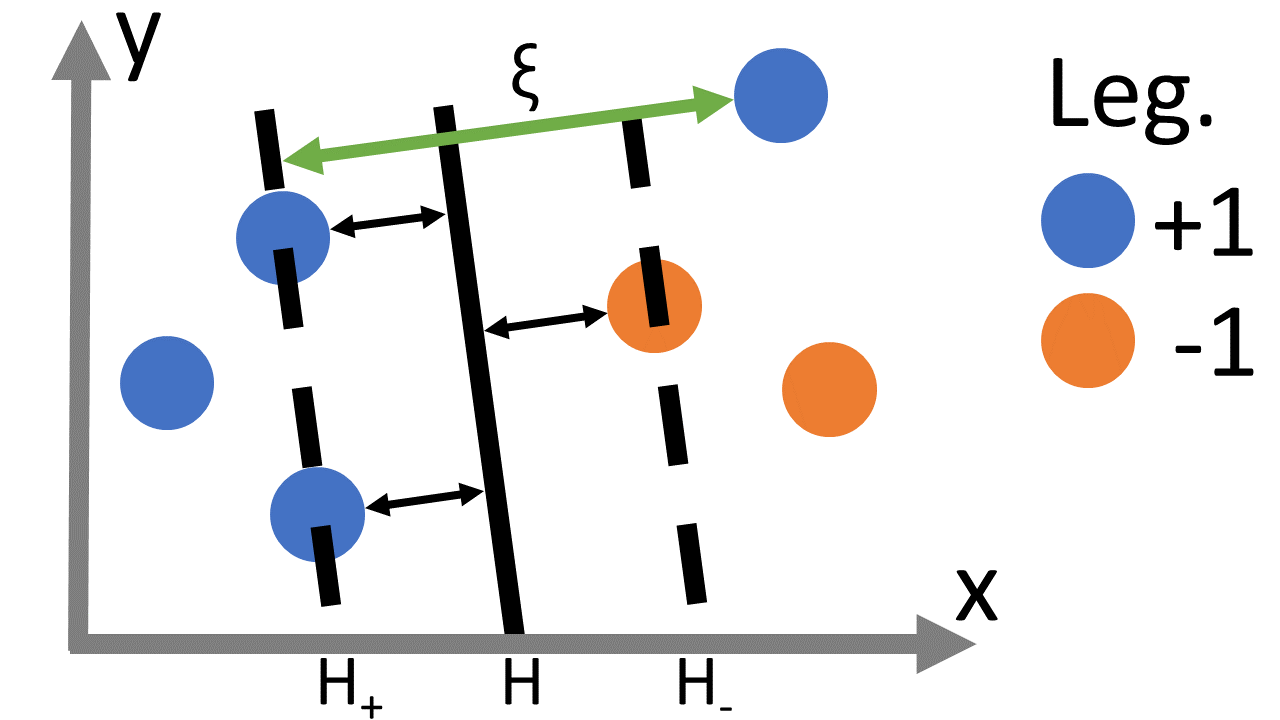
\includegraphics[width=\textwidth]{PowerPoint/Folie18.png}
                    % \caption{Beispiel eines Training-Sets}
                    \label{Schlupf:fig_1}
                }
            \end{figure}
        \end{minipage}
        \hfill
        \begin{minipage}{0.4\textwidth}
            \begin{itemize}
                \item Schlupfvariable $\xi$ zum Ausgleich falscher Messwerte
            \end{itemize}
        \end{minipage}
    \end{figure}

    \begin{itemize}
        \item GC:
            \begin{align*}
                & y_i ( \boldsymbol{w}^T \boldsymbol{x}_i + b ) \geq 1 - \xi_i \quad \forall \boldsymbol{x}_i \in S & \xi_i \geq 0\\
            \end{align*}
        \item Minimierungsproblem:
            \begin{align*}
                &\min_{\boldsymbol{w}, b, \boldsymbol{\xi}} \frac{1}{2} \Vert \boldsymbol{w} \Vert^2 + C \sum_i \xi_i \\
                &\text{u.d.N. } y_i ( \boldsymbol{w}^T \boldsymbol{x}_i + b ) \geq 1 - \xi_i \land \xi_i \geq 0 \\
            \end{align*}
    \end{itemize}
\end{frame}

%%%%%%%%%%%%%%%%%%%%%%%%%%%%%%%%%%%%%%%%%%%%%%%%%%%%%%%%%%%%%%%%%%%%%%%%%%%%%%%%
% Folie 15: Zusammenfassung
%%%%%%%%%%%%%%%%%%%%%%%%%%%%%%%%%%%%%%%%%%%%%%%%%%%%%%%%%%%%%%%%%%%%%%%%%%%%%%%%
\begin{frame}
    \frametitle{Zusammenfassung}

    \begin{itemize}
        \item Kanonische Hyperebene:
            \begin{align*}
                \boldsymbol{w}^T \boldsymbol{x} + b = 0
            \end{align*}
        \item Gesucht: Parameter $\boldsymbol{w}$ und $b$
        \item Langange Multiplikatoren:
            \begin{align*}
                & \max_{\boldsymbol{w}, b, \boldsymbol{\alpha}} L = \sum_i \alpha_i - \frac{1}{2} \sum_i \sum_j \alpha_i \alpha_j y_i y_j \boldsymbol{x}_i^T \boldsymbol{x}_j \\
                & \boldsymbol{w} = \sum_i \alpha_i y_i \boldsymbol{x}_i \\
                & \sum_i \alpha_i y_i = 0 \\
            \end{align*}
        \item Entscheidungsfunktion $h$:
            \begin{align*}
                h(\boldsymbol{x}) = \begin{cases}
                    +1 & \sum_i \alpha_i y_i \boldsymbol{x}_i^T \boldsymbol{x} + b \geq 0 \\
                    -1 & \sum_i \alpha_i y_i \boldsymbol{x}_i^T \boldsymbol{x} + b \leq 0 \\
                \end{cases}
            \end{align*}
    \end{itemize}
\end{frame}


%%%%%%%%%%%%%%%%%%%%%%%%%%%%%%%%%%%%%%%%%%%%%%%%%%%%%%%%%%%%%%%%%%%%%%%%%%%%%%%%
% Quellen
%%%%%%%%%%%%%%%%%%%%%%%%%%%%%%%%%%%%%%%%%%%%%%%%%%%%%%%%%%%%%%%%%%%%%%%%%%%%%%%%
% \begin{frame}
%     \frametitle{Quellen}

%     \nocite{*}
%     \printbibliography
% \end{frame}
